\documentclass[12pt, a4paper]{article}
\usepackage[utf8]{inputenc}
\usepackage{graphicx}
\usepackage{geometry}
\usepackage{booktabs}
\usepackage{hyperref}
\usepackage{amsmath}
\usepackage{cite}
\usepackage{pmboxdraw}
\usepackage{minted}

% Page geometry
\geometry{a4paper, margin=0.5in}

\title{
    \textbf{GPU Accelerated Synthetic Human Voice Narration with GUI}
}


\author{Karthik M Dani \and Darshan S K}

\date{\today}



\begin{document}

\maketitle
\tableofcontents
\newpage

\section{Abstract}

This project leverages the power of modern deep learning techniques \cite{arxivAttentionNeed} and GPU acceleration to generate high-quality, human-like synthetic voice narration from input text. The system employs the Bark deep learning model \cite{huggingfaceSunobarksmallHugging}, a state-of-the-art transformer-based architecture for text-to-speech (TTS) tasks. The software uses Python, PyTorch \cite{NEURIPS2019_bdbca288}, and the Transformers library to generate speech, while providing a user-friendly graphical interface using the Tkinter library \cite{lundh1999introduction}. The system can efficiently process large amounts of text by chunking input, handling GPU-based processing, and managing audio output. This report describes the structure and key components of the project, as well as its performance and potential improvements.

\section{Introduction}

Text-to-speech synthesis involves converting written text into spoken words, and recent advancements in deep learning have enabled the creation of highly natural-sounding speech models. This project focuses on developing a GPU-accelerated text-to-speech (TTS) system that mimics human-like narration. The primary goal is to enhance the process of generating spoken text, incorporating features such as chunking large texts, leveraging GPU for speedup, and integrating an interactive graphical user interface (GUI).

Key objectives of the project:

\begin{itemize}

\item Implement text-to-speech synthesis using the Bark model.

\item Utilize GPU acceleration for faster processing.

\item Develop a user-friendly GUI for text input and speech generation.

\item Enable efficient handling of large texts through chunking.

\end{itemize}

\section{Background}

Text-to-speech synthesis has been studied for several decades, with early methods relying on concatenating recorded human speech samples. Recent developments in machine learning, particularly deep neural networks, have allowed for more natural-sounding synthetic voices. The Bark model, used in this project, is a generative TTS model that employs transformers to produce high-quality speech.

Key components:

\begin{itemize}

\item \textbf{Bark Model:} A pretrained deep learning model that generates speech from text using a large transformer-based architecture.

\item \textbf{Chunking:} Large input texts are broken into smaller segments, called chunks, to fit within model constraints (memory and processing limits). This allows for the efficient handling of lengthy inputs.

\end{itemize}

\section{Methodology}

The project involves several stages: model loading, text chunking, speech generation, and output handling. Below is a step-by-step explanation of the implementation:
 
\subsection{Loading the Model}

The Bark model is loaded using the Hugging Face transformers library \cite{huggingfaceHuggingFace}. The model is trained for high-quality text-to-speech generation and is loaded onto the available GPU (if available) for faster processing.

\begin{minted}{python}

model = BarkModel.from_pretrained("suno/bark-small")
device = "cuda:0" if torch.cuda.is_available() else "cpu"
model = model.to(device)
processor = AutoProcessor.from_pretrained("suno/bark")

\end{minted}

Here, the BarkModel is initialized from the Hugging Face repository, and the processor is used to prepare the input text in the required format.

\subsection{Chunking the Text}

To manage long text inputs that might exceed model limitations, the text is split into smaller chunks. Each chunk contains up to max\_chunk\_size words, and this approach prevents memory overflow during processing. The chunk\_text\_by\_words function takes care of this.

\begin{minted}{python}

def chunk_text_by_words(text, 
max_chunk_size=max_chunk_size):
    words = text.split()
    chunks = [" ".join(words[i:i + max_chunk_size]) 
    for i in range(0, len(words), max_chunk_size)]
    return chunks

\end{minted}

The chunks are iterated through during the speech generation process.

\subsection{Speech Generation}

Each chunk of text is processed using the BarkModel to generate the corresponding speech. The text is passed through the processor, and the model’s generate function is called to produce the speech, which is then saved as an audio file.

\begin{minted}{python}

inputs = processor(chunk, voice_preset=voice_preset)
speech_output = model.generate(**inputs.to(device))
speech_outputs.append(speech_output[0].cpu().numpy())

\end{minted}

The speech output is concatenated from the individual chunks and saved in \texttt{.wav} format using the scipy.io.wavfile.write function.

\subsection{GUI Implementation}

The user interface is built with Tkinter, a Python library for creating graphical user interfaces. It provides a text input area for the user to enter the text to be converted to speech, a "Generate Speech" button to trigger the process, and a progress message that updates the user on the ongoing process.

\begin{minted}{python}

root = tk.Tk()
input_text = tk.Text(root, wrap=tk.WORD, 
height=15, font=("Arial", 12), bg="#1E1E1E", fg="white", insertbackground="white")
generate_button = ttk.Button(root, 
text="Generate Speech", command=on_generate_click)


\end{minted}

A simple and effective design was chosen to focus on functionality and ease of use. The application is run in a loop using root.mainloop() to keep the window active.

\begin{figure}[h!]
\centering
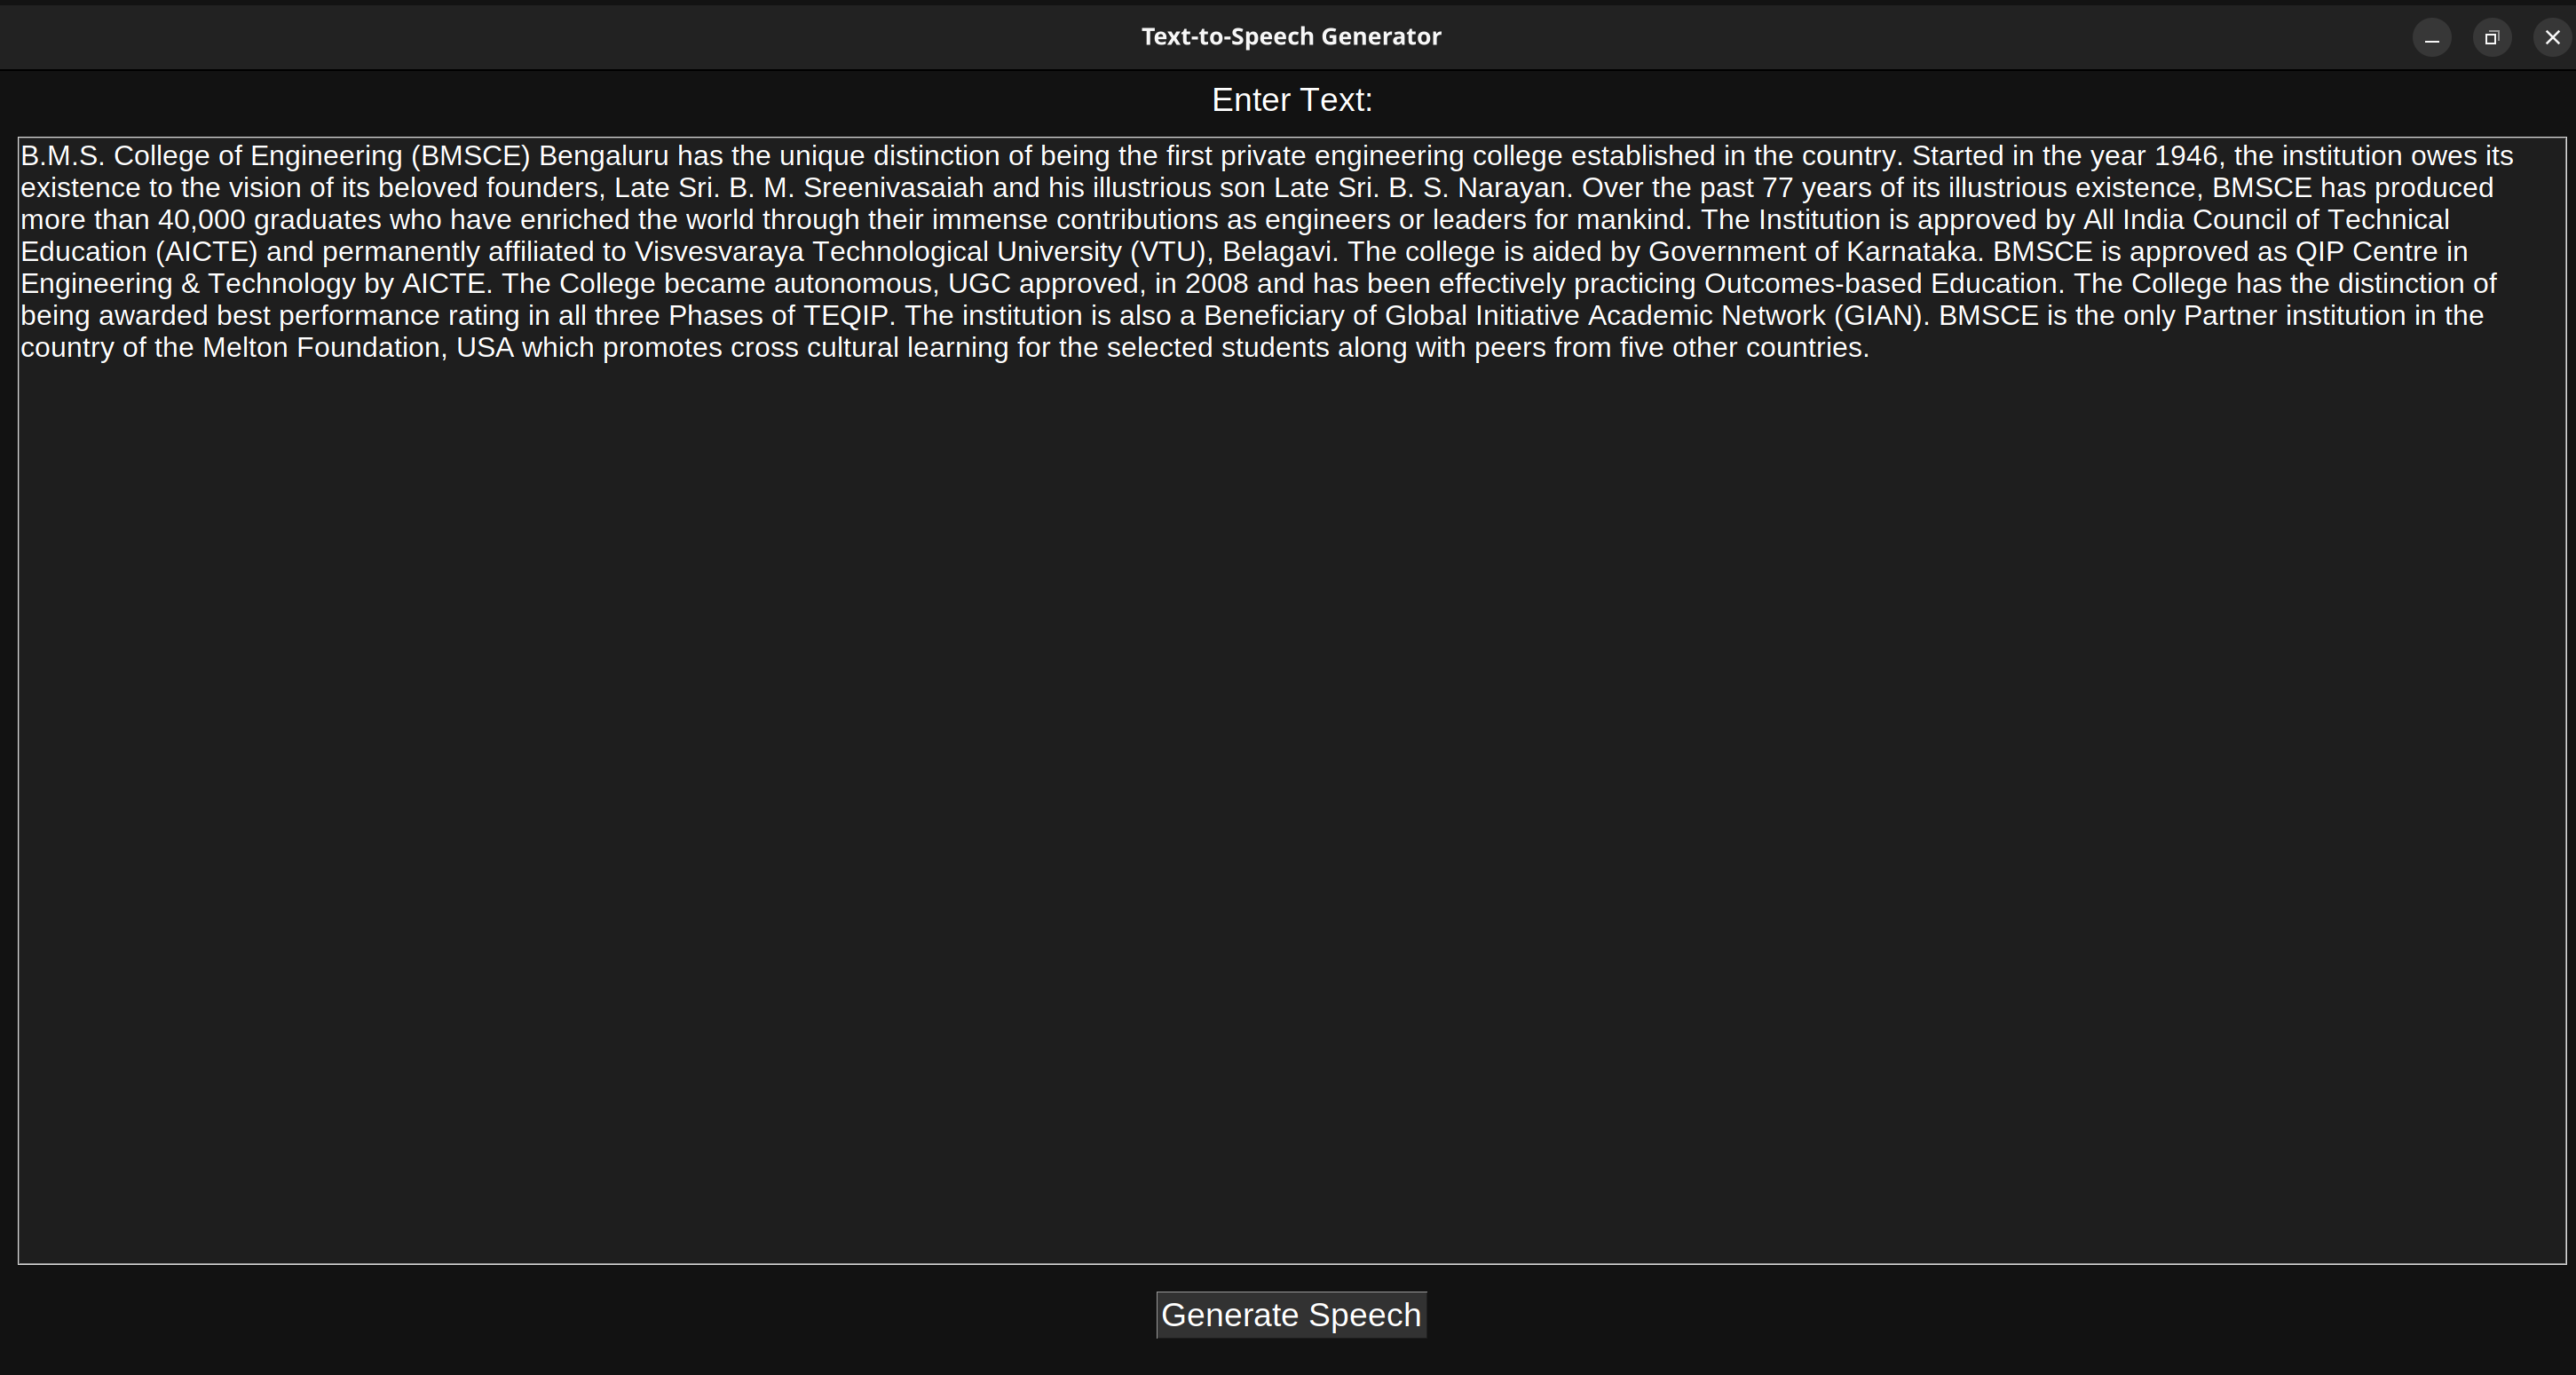
\includegraphics[width=0.8\textwidth]{figures/gui.png}
\caption{GUI of the Application with an area to enter sentences to produce audio}
\label{fig:test_results}
\end{figure}

\section{Code}

\begin{minted}{python}

import tkinter as tk
from tkinter import ttk, filedialog, messagebox
import torch
from transformers import AutoProcessor, BarkModel
import numpy as np
import scipy.io.wavfile

# Load model and processor
model = BarkModel.from_pretrained("suno/bark-small")
device = "cuda:0" if torch.cuda.is_available() else "cpu"
model = model.to(device)
processor = AutoProcessor.from_pretrained("suno/bark")

voice_preset = "v2/en_speaker_6"
max_chunk_size = 22

# Function to chunk text
##
# This function chunks the input text into smaller pieces, 
# each containing up to a specified number of words.
# The chunks are returned as a list of strings, which can be 
# processed individually by the TTS model.
#
# @param text The input text to be split into chunks.
# @param max_chunk_size The maximum number of words allowed in 
# each chunk (default is 22).
# @return A list of text chunks, each containing a subset of 
# the original text.
def chunk_text_by_words(text, max_chunk_size=max_chunk_size):
    words = text.split()
    chunks = [" ".join(words[i:i + max_chunk_size]) 
              for i in range(0, len(words), max_chunk_size)]
    return chunks

# Function to process text and generate speech
##
# This function generates speech from the input text 
# using the Bark TTS model.
# It processes the text by splitting it into chunks, 
# converting each chunk into speech, and concatenating 
# the results. The final output is saved as a WAV audio file.
#
# @param text The input text to be converted to speech.
# @param output_path The path where the generated audio 
# will be saved as a WAV file.
def generate_speech(text, output_path):
    try:
        text_chunks = chunk_text_by_words(text)
        speech_outputs = []

        # Loop through text chunks and generate 
        # speech for each
        for i, chunk in enumerate(text_chunks):
            progress_message.set(
                f"Processing chunk {i + 1}/{len(text_chunks)}: {chunk}")
            # Update the GUI to reflect the current progress
            root.update()  

            # Process input chunk for TTS model
            inputs = processor(chunk, voice_preset=voice_preset)
            # Generate speech output from model
            speech_output = model.generate(**inputs.to(device)) 
            # Convert to numpy array and store in list
            speech_outputs.append(speech_output[0].cpu().numpy()) 

        # Concatenate all speech outputs into a single audio
        concatenated_output = np.concatenate(speech_outputs)
        sampling_rate = model.generation_config.sample_rate

        # Save the generated speech to a WAV file
        scipy.io.wavfile.write(output_path, rate=sampling_rate, 
                               data=concatenated_output)

        progress_message.set("Audio generation complete! Saved to: " + output_path)
        messagebox.showinfo("Success", f"Audio saved to {output_path}")
    except Exception as e:
        progress_message.set("Error during processing.")
        messagebox.showerror("Error", str(e))

# Function to handle generate button click
##
# This function is triggered when the user clicks the 
# "Generate Speech" button.
# It retrieves the input text, prompts the user to choose 
# a save location, and calls the generate_speech function.
#
# @return None
def on_generate_click():
    text = input_text.get("1.0", tk.END).strip()
    if not text:
        messagebox.showwarning("Input Required", 
                               "Please enter some text to generate speech.")
        return

    # Prompt user to select the location to save the 
    # generated audio
    output_path = filedialog.asksaveasfilename(
        defaultextension=".wav",
        filetypes=[("WAV files", "*.wav")],
        title="Save Audio File"
    )

    if output_path:
        progress_message.set("Starting audio generation...")
        # Update the GUI before processing
        root.update()  
        # Generate the speech and save it
        generate_speech(text, output_path)  

# Create GUI
##
# This section sets up the graphical user interface using Tkinter. 
# It contains a text input field for entering text,
# a "Generate Speech" button to trigger the speech generation, 
# and a progress label to display the current status.
root = tk.Tk()
root.title("Text-to-Speech Generator")
root.geometry("1000x600") 
# Dark theme background
root.configure(bg="#121212")  

# Input text area
input_label = ttk.Label(root, text="Enter Text:", background="#121212", 
                        foreground="white", font=("Arial", 14))
input_label.pack(pady=10)

input_text = tk.Text(root, wrap=tk.WORD, height=15, font=("Arial", 12), 
                     bg="#1E1E1E", fg="white", insertbackground="white")
input_text.pack(padx=20, pady=10, fill=tk.BOTH, expand=True)

# Generate button
generate_button = ttk.Button(root, text="Generate Speech", 
                             command=on_generate_click, style="Custom.TButton")
generate_button.pack(pady=20)

# Progress message
progress_message = tk.StringVar()
progress_label = ttk.Label(root, textvariable=progress_message, 
                           background="#121212", foreground="lightblue", 
                           font=("Arial", 12, "italic"))
progress_label.pack(pady=10)

# Style configuration for custom button appearance
style = ttk.Style()
style.configure("Custom.TButton", font=("Arial", 14), 
                background="#323232", foreground="white")
style.map("Custom.TButton", background=[("active", "#505050")])

# Start GUI loop
##
# This starts the Tkinter event loop, 
# which allows the GUI to run and respond to user actions.
root.mainloop()


\end{minted}

\section{Results}

Upon execution, the system allows the user to input text, which is processed and converted into a synthetic voice narration. The user can save the output as a .wav file. GPU acceleration ensures that larger text inputs are processed relatively quickly compared to CPU-only implementations.

\begin{figure}[h!]
\centering
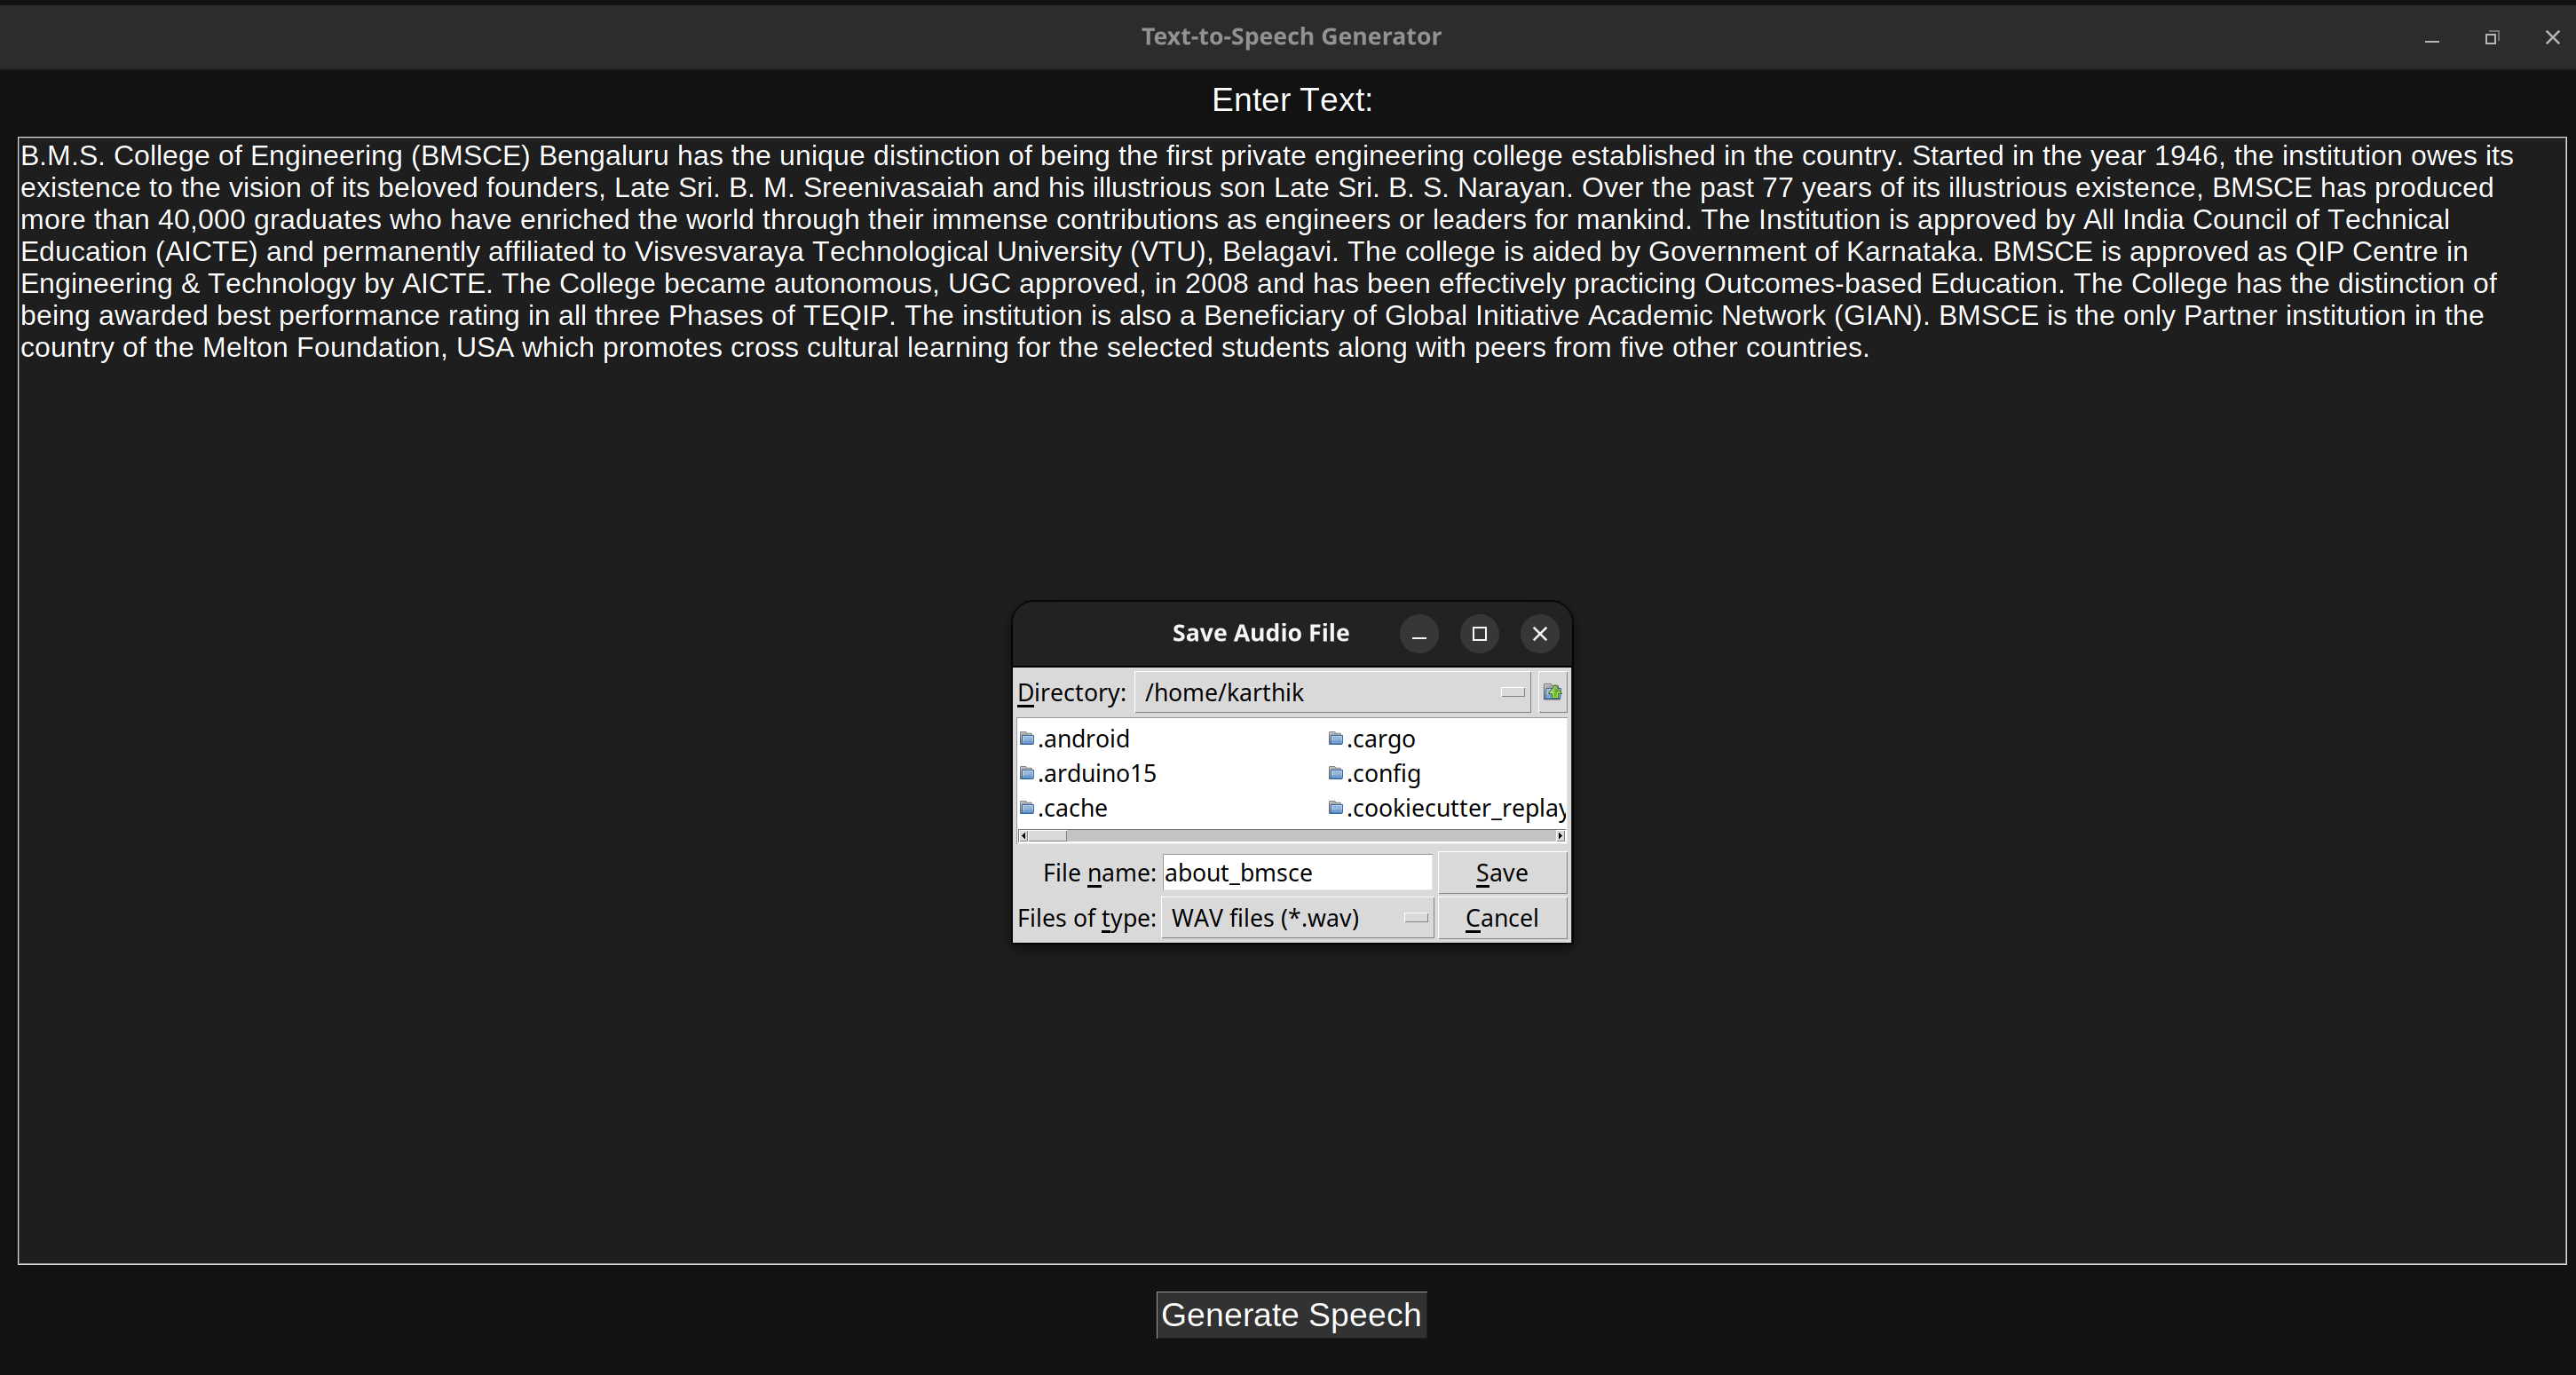
\includegraphics[width=0.8\textwidth]{figures/about.png}
\caption{Prompting the location to save the generated audio file}
\label{fig:test_results}
\end{figure}

\begin{itemize}

\item Text is chunked into smaller segments to manage memory usage and processing power.

\item The progress is displayed dynamically through the GUI.

\item The synthesized speech is of high quality, similar to human speech, thanks to the Bark model's transformer-based architecture.

\end{itemize}

\begin{figure}[h!]
\centering
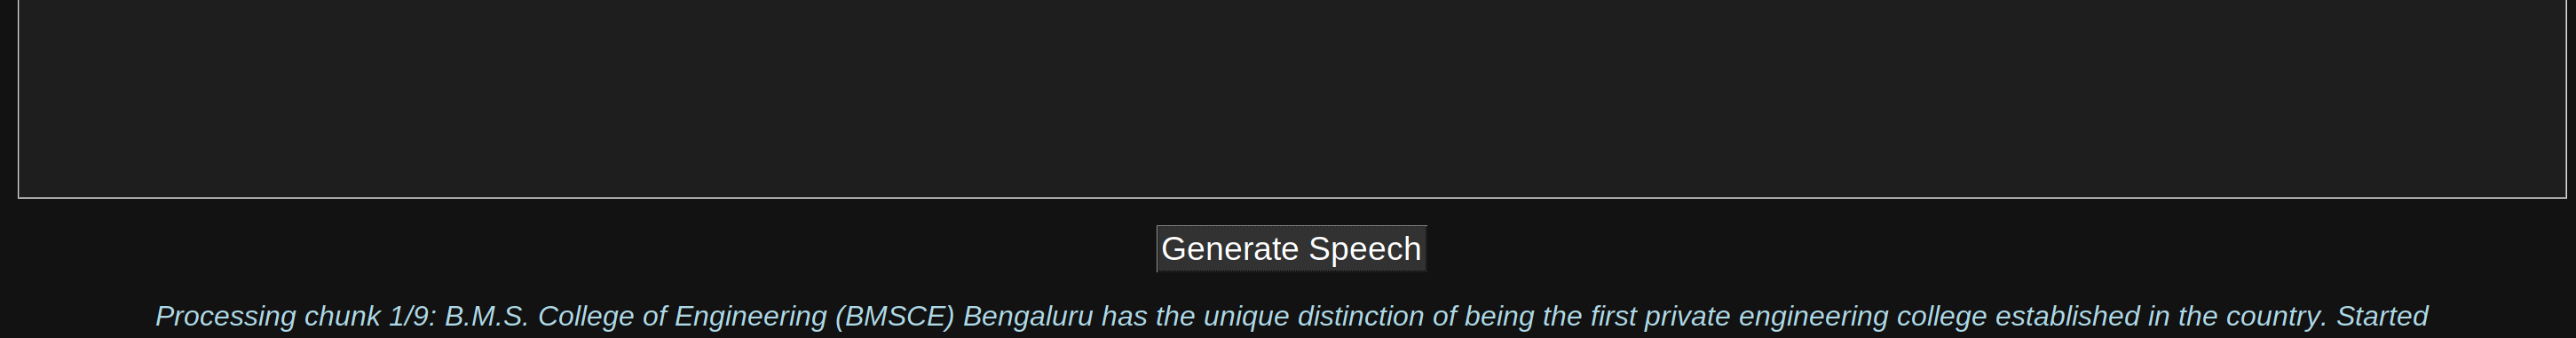
\includegraphics[width=0.8\textwidth]{figures/status.png}
\caption{Progress of the audio generation}
\label{fig:test_results}
\end{figure}


\section{Analysis}

\subsection{Performance}

\begin{itemize}

\item \textbf{Speed:} The system leverages GPU acceleration, which significantly improves processing speed, especially when dealing with large text inputs. On a GPU-enabled machine, speech generation for several paragraphs can take less than a minute.

\item \textbf{Chunking Efficiency:} The chunking method ensures that even long documents can be processed without running into memory limitations.

\end{itemize}


\subsection{Limitations}

\begin{itemize}

\item \textbf{GPU Dependency:} The performance is heavily dependent on the availability of a compatible GPU. Users without a GPU may experience slower processing times.

\item \textbf{Text Preprocessing:} While the chunking approach works well for most cases, certain edge cases (e.g., special characters, complex punctuation) may require further text preprocessing.

\end{itemize}


\subsection{Potential Improvements}

\begin{itemize}

\item \textbf{Text Normalization:} Implementing text normalization algorithms to handle complex characters or inconsistent formatting can improve the system's robustness.

\item \textbf{Voice Variety:} The system can be extended to support multiple voices or accents, making it more flexible for different applications.

\item \textbf{Performance Optimization:} Optimizing the chunking mechanism for better memory management and parallel processing could further speed up the system.

\end{itemize}


\section{Conclusions}

This project successfully integrates deep learning-based text-to-speech synthesis with GPU acceleration and a user-friendly interface. By using the Bark model and leveraging GPU hardware, it produces high-quality synthetic speech quickly and efficiently. While there are areas for improvement, particularly in handling various text formats and expanding voice options, the current implementation demonstrates a solid foundation for building advanced TTS systems.



\section{Acknowledgement}

We thank Dr. Niranjan K R sir for suggesting improvements in the project and also considering this real world project for evaluation that allow us to contribute.
 
\bibliographystyle{unsrt} % or any style you prefer (e.g., abbrv, alpha, etc.)
\bibliography{references} % 'references' is the name of your .bib file (no need to add .bib extension)


\end{document}
